\documentclass[a4paper,11pt]{article}

\usepackage{acl-ijcnlp2009}

\usepackage{epsfig} \usepackage{times} \usepackage{url} \usepackage{latexsym}

\usepackage{multirow}

\title{Self Organizing Maps in a Learning Game}

\author{Keith Stevens \\ University of California, Los Angeles \\
kstevens@cs.ucla.edu}

\date{}

\begin{document}

\maketitle

\section{Introduction}
%hypothesis goes here, approach, claims and goals also go here.
Acquiring the first aspects of language in artificial agents is a problem that
has been addressed by a variety of approaches.  There are symbolic approaches
which use logical inferences to deduce which object a word refers to
\cite{Siskind} and approaches which use simple decision trees and predicate
logic to ground the meaning of a word \cite{GoldNico}.  There are also
statistical approaches which utilize bayesian statistics  and probabilities to
compute the likelihood of a word grounding to a particular object based on it's
usage \cite{FazlyProbRefUn,SmithCommSystem,VogtSocial}.  Each of these
approaches have worked to tackle a central issue, the presence of referential
uncertainty.  

Referential uncertainty is a term describing the situation where a word can be
heard, and several objects could be present to a young learning agent.  The
agent would then have to decide which object the word most likely refers too.
This is best described by Quine \cite{Quine} with his ``gavagi`` problem, where
an anthropologist is traveling with a tribe of people speaking a foreign tongue,
and suddenly one of them points to a rabbit and speaks ``gavagi``.  Knowing no
words for this language so far, the anthropologist must guess which object the
word refers to, usually by observing multiple uses of the word, in different
contexts.  Both symbolic and statistical approaches have relied on the key
assumption that words are eventually used in enough contexts to clarify their
meaning.

Recently, a connectionist model has been introduced which models early word
acquisition by use of several connected self organizing maps
\cite{LiDevLex,MiikDisLex}.  The DevLex system has the appealing ability to
model a growing lexicon \cite{LiDevLex}, which can be challenging in
connectionist systems due to catastrophic interference, by training connections
between the two maps with pairs of semantic representations and phonological
representations.  One issue mentioned by the authors earlier in \cite{FarkasWcd}
is that connectionist systems tend to learn based on unrealistic data, and
address this problem by taking incorporating word cooccurence information into
the semantic representations based on the agents current lexicon.  The one key
feature missing from this system is the incorporation of referential uncertainty
when learning.

This project introduces a combination of a simplified version of the DevLex
architecture \cite{LiDevLex}, and a simple learning game frequently used for
bootstrapping lexical groundings in statistical agents
\cite{VogtLearningSim,VogtSocial}.  There are two key challenges in this
project.  First, can agents using self organizing maps correctly agree on a
language when no language currently exists when there is no referential
uncertainty?  Second, can these agents, or an enhancement of these agents,
handle referential uncertainty when learning?

\section{Overview and the Learning Game}
%describe the hypotheses in more detail.
A simulation of how humans acquire their first words would present a situation
where an agent which has a well defined lexicon speaks about the world with a new
agent, but this well established agent would have to be designed by hand.  As
such, an approximation of early word acquisition has been used which allows new
agents to bootstrap their lexicons through simple learning games
\cite{VogtLearningSim,VogtSocial}.  In some respects, this approximation is
similar to young children interacting with each other and naming unfamiliar
objects. 

\begin{figure} \center 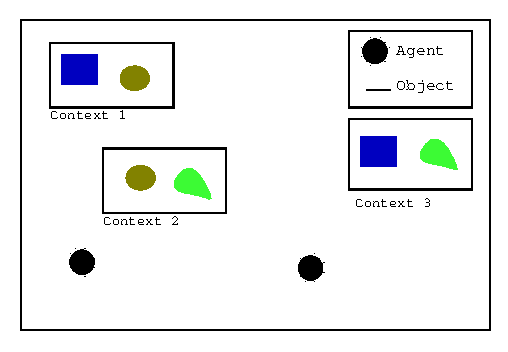
\includegraphics[width=.49\textwidth]{game-env.eps}
\caption{Sample game environment with 2 agents.} \label{fig:game-env}
\end{figure}

Each learning game has the following basic steps:

\begin{enumerate}

\item A speaker is chosen.

\item A speaker chooses a set of objects which will be the context of the
conversation.  It then selects one of the objects within the context to be the
focus object of the learning game.

\item The speaker speaks some phrase which best describes the focus object.

\item If the speaker is unable produce a phrase with confidence, the
speaker selects a word at random from a global lexicon.

\item The hearer sees the context objects, and hears the phrase spoken.  

\item The hearer tries to deduce which object in the context the phrase
corresponds to.

\end{enumerate}

There are three basic versions of a simple learning game introduced in
\cite{VogtLearningSim}, which are each progressively more difficult to handle.

\begin{enumerate}

\item Observation Game: The speaker informs the hearer of the focus object before
speaking.

\item Guessing Game: The hearer is not informed of the focus object, but can
point to the object it guesses to be the focus object, and the speaker can either
confirm or correct the guess.

\item Selfish Game: The hearer is not informed of the focus object, and makes no
response during the learning game.

\end{enumerate}

The Observation Game is of little interest for this project since this is akin
to telepathicly telling each agent what the mapping should be, and side steps
the presence of referential uncertainty altogether.  The Guessing Game is of
some interest, since this represents either a correction or a reward for the
hearing agent after making a guess.  The last version of the learning game, the
Selfish Game, is of the most interest, since if the speaker has a well defined
lexicon, this would be a close simulation of a parent speaking about the world,
with a child passively overhearing the conversation and attempting to map the
phrases to observable objects.  In the current model of bootstrapping a lexicon,
it still is of interest, as it could be considered to be a simulation of agents
developing a pidgin language, or children deciding new names for objects the are
unfamiliar with, while still exhibiting the most significant challenges in
meaning learning.

One key issue in both games is deciding when each the speaker and hearer should
learn a mapping from a word to an observation.  The speaker will always have an
advantage because the focus object is known to the agent, so in both the
Guessing Game and the Selfish Game, the speaker can learn a mapping as soon as a
word is produced for the focus object.  The hearer on the other hand has options
for when to learn based on the game type.  In the Guessing game, learning could
happen before making a guess, after making a guess, or both before and after
making the guess.  The simplest approach, which fully utilizes the structure
of the game, is to learn after the hearer makes a guess, and learn to
associate the current context with the focus object so that in later games,
the context will allow the hearer to correctly guess the object. In the
Selfish Game, the agent has only one option for learning, the time of
observation.

It is my main hypothesis that a agents which use only a simple self organizing
map should be capable of converging upon a small artifical language in a series
of Selfish Games without referential uncertainty. My second hypothesis is that
once referential uncertainty is introduced, the self organizing map alone will
be insufficient, and would need some additional mechanism, yet should still be
feasible with the Selfish Game.  Third, by complicating the self organizing map
with additional maps, a langauge can be determined with the Selfish Game without
referential uncertaintly.  Finally, agents using several connected maps not be
capable of reaching a language with a series of Selfish Games with the presence
of referential uncertainty.

\section{Architecture}

%architecture goes here, along with description of software packages used, and
%the current status of each module.
In order to accommodate multiple experiments, the connectionist architecture has
a simple, modular design.  There are two standard Self Organizing Maps, one for
semantic representations, and one for phonological representations, where all
nodes in one map are connected to all nodes in the other map.  Each node in
the two maps has a meaning vector, and an activation associated with it.  Each
connection between nodes from the semantic and phonological map has a
uni-directional weight.  Each map also monotonically decreases the size of the
neighborhood over time.  Lastly, each node in the semantic map has a set
of attenion weights which will vary based on variation of semantic meanings
mapped to the particular node.  Figure \ref{fig:arch} provides a graphical
description of this architecture.

\begin{figure} \center 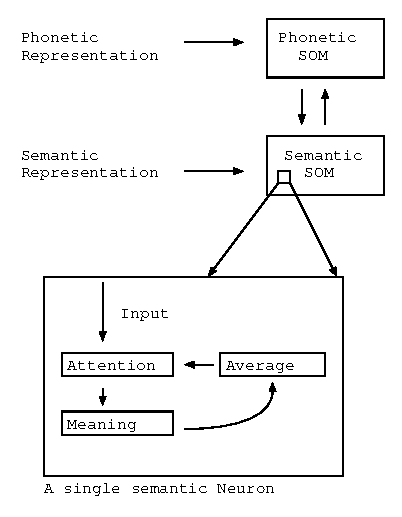
\includegraphics[width=.49\textwidth]{arch.eps}
\caption{Architecture of a single learning agent} \label{fig:arch} \end{figure}

Aside from the attentional weights maintained for each node, the basic
structure of the two self organizing maps is derived from
\cite{LiDevLex,MiikDisLex}, and is summarized as follows.

When a new input stimulus, $x$ is presented to the map for training, a winning
node is found by finding the node $k$ whose meaning vector, $m_k$ has the
smallest euclidian distance to $x$.  Neuron $k$ will then be the center of all
updates done to the map, with $N_k$ being the set of neighbors to $m_k$.  The
meaning vector of each node in a map, is then updated according to the a
slight modification to the standard SOM update scheme:

{\small \begin{equation}\label{eq:meaning_weight}
m_{ij}(t+1) = m_{ij}(t) + N(i)*\alpha(t)[atten_{ij}(t)x_j - m_{ij}(t)]
\end{equation} }

where $N(i)$ is 1 if node $i \in N_c$ and 0 otherwise, $\alpha(t)$ is the
learning rate which decreases monotonically, and $atten_{ij}(t)$ is the
attentional weight of each feature in a semantic representation for this node.
This attentinonal weight is defined to be:

\begin{equation}\label{eq:atten}
att_{ij}(t) = 1 / (1 + variance_{ij}(m_{ij}))
\end{equation}

The variance of each feature is maintained as a rolling variance, along with a
rolling average based on the techniques presented in
\cite{mints93rollingvariance}.

To maintain the unidirectional link between nodes of each map, the activation of
each node must first be computed, where the highest activation will be centered
around the winning node, and a spread of activation within the node's
neighborhood is produced in each map.  Formally, this activation is computed as:

\begin{equation}\label{eq:act}
a_i = N(i)*(1 - \frac{||\textbf{x} - \textbf{m$_i$}|| - d_{min} }{d_{max} -
d_{min}})
\end{equation}

where $d_{min}$ and $d_{max}$ are the smallest and largest meaning distances
within $N_c$.  With these activations, the uni-directional hebbian weights are
updated with:

\begin{equation}\label{eq:heb_weight}
w_{kl}(t+1) = w_{kl}(t) + \alpha(t+1)a_k^Sa_l^D
\end{equation}

which maintains a two dimensional matrix of weights, and is then normalized
according to row length normalization.  When training, a string representation
of the word is also presented to the system.  When the phonological map 
is present, the word is mapped to the winning node in the phonological map.
Otherwise, the word is mapped to the winning node in the semantic map.


For production, a winning node is produced in the map which receives input by
again selecting the node whose meaning vector has the smallest euclidian
distance to the input $x$.  The activation for the nodes in this map are again
computed using Equation \ref{eq:act}.  The activations in the output map are
produced by propogating the source activation over the hebbian links using:

\begin{equation}\label{eq:prop}
a_l^D = \sum_k w_{kl}a_k^S
\end{equation}

And the output produced by the output map is decided by the node which has the
highest activation.

In production, if the node which determines what phrase to speak is selected with a
confidence less than some threshold, a new word is selected, and the agent
trains itself to map the semantic input to the phonological input of the new
word.

Lastly, the neighborhood $N_k$ is defined by

\begin{equation}\label{eq:neighbors}
N_k = \{ i \:| \:|| \textbf{loc$_i$} - \textbf{loc$_k$} || \leq 50\exp(\frac
{-t}{177})\}
\end{equation}

\subsection{Configurations to the system}

Since several configurations of learning need to be tested, several of the
components can be disconnected and turned off.  The attentional weights can be
shut off completely, simply by initializing all weights to 1 and not using
Equation \ref{eq:atten}.  Similarly, phonological mappings can be shut off by
ignoring Equations \ref{eq:act}, \ref{eq:heb_weight} and \ref{eq:prop}.  In
this configuration, production is simply done by producing the word mapped to
the winning node in the semantic map.

\section{Input}

\begin{center}
  \begin{table*}
    \begin{tabular}[t] { | l | c | c | }
      \hline
      Word & Category & Vector \\
      \hline
      ball & Toys & \includegraphics[width=.80\textwidth]{ball.ppm} \\
      cheese & Food \& Drink & \includegraphics[width=.80\textwidth]{cheese.ppm} \\
      juice & Food \& Drink &\includegraphics[width=.80\textwidth]{juice.ppm} \\ 
      milk & Food \& Drink &\includegraphics[width=.80\textwidth]{milk.ppm} \\ 
      pants & Clothing & \includegraphics[width=.80\textwidth]{pants.ppm} \\
      sock & Clothing &\includegraphics[width=.80\textwidth]{sock.ppm} \\
      \hline
    \end{tabular}
    \caption{Sample vectors for semantic representations}
    \label{tb:semantics}
  \end{table*}
\end{center}

\begin{center}
  \begin{table}
    \begin{tabular}[t] { | l | c | }
      \hline
      Word & Vector \\
      \hline
      a &  \includegraphics[width=.40\textwidth]{a.ps} \\
      ai &  \includegraphics[width=.40\textwidth]{ai.ps} \\
      an & \includegraphics[width=.40\textwidth]{an.ps} \\ 
      ang & \includegraphics[width=.40\textwidth]{ang.ps} \\ 
      ao & \includegraphics[width=.40\textwidth]{ao.ps} \\
      ba & \includegraphics[width=.40\textwidth]{ba.ps} \\
      \hline
    \end{tabular}
    \caption{Sample vectors for phonetic representations}
    \label{tb:phono}
  \end{table}
\end{center}

%general io and specific examples goes here.
Two forms of input need to be fed into the system, semantic representations and
phonological representations.  Additionally there is a fixed global lexicon of words
which is accompanied by the phonological representations.  The phonological
vectors are a low dimensional feature vector representing a single word.  The
semantic vector represents the features in a single word.  When referential
uncertainty is introduced to the learning games, the semantic vectors of each
object in the selected context are summed together to produce a single feature
vector which is used as input to the hearer.

For phonetics,
vectors are produced from the PatPho system \cite{LiPatPho}.  These vectors have 15
real valued features which are produced based on how each word fits into a
syllable template.  PatPho vectors for 401 chinese words are used with the
pinyin romanization for the string form of each word.  A sample of these vectors
can be seen in Table \ref{tb:phono}

The semantic vectors correspond to the objects placed in the learning environment.
For these semantic representations, initially 60 vectors, each with 60 real valued
features, were randomly generated.  In each random vector, 3 random features were
randomly assigned a value between 0 and 1.  These random vectors had no underlying
patterns within them.

The other set of semantic vectors are built using a feature generation system
\cite{HarmWordNetFeature}.  This feature generation system first builds binary
features for the provided words based on information in the WordNet taxonomy.
Since these binary feature vectors are of a high dimension, they are reduced
using random mapping, This process is also used for the semantic vectors used in
DevLex \cite{LiDevLex}.  The 60 words used for generating vectors were taken
from the vocabulary from the MacArthur–Bates Communicative Development
Inventories (CDI) \cite{DaleCDI}.  This list is a collection of words learned by
toddlers in early stages of word acquisition.  The 60 words selected were the
first 60 in this list when sorted according to age the word is acquired, and
thus the earliest words acquired by toddlers.  These words are approximately the
first 60 words used in \cite{LiDevLex}.

\section{Experiment and result}
%describe the results
For this project, the experiment is to run a series of learning games with a
small number of learning agents to determine whether or not a population of simple connectionist
agents can agree on a language.  Several configurations of agents are run:

{\small
\begin{enumerate}

\item Agents use only a semantic map, with no attentional learning.

\item Agents use only a semantic map with attentional learning.

\item Agents ues both maps with no attentional learning.

\item Agents use both maps with attentional learning.

\end{enumerate}
}

In addition to these configurations for agents, the learning environment is also
modified to produce context of size 4 (presence of referential uncertainty), or
produce contexts of size 1 (no referential uncertainty).  To address my
hypoheses, only Selfish Games are run, with 2 agents in the population.

To evaluate each configuration, two key metrics are used.  First is language
convergence, which determines how many objects all the agents are capable of
agreeing on a
single term.  Second is the rate of homonymy, measuring how many objects are
referred to by each word.  If both convergence and homonym are high, then the
agents have developed a vague and unusable language.  The ideal language should
have high convergence and low homonymy.  

\begin{center}
\begin{table}
\begin{tabular}[ht]{ | c | c | c | c | c |}
\hline
 & \multicolumn{2}{|c|}{No Context} & \multicolumn{2}{|c|}{Wtih Context} \\
 \hline
 Configuration & Con & H& Con & H \\
 \hline
 1 & 1.0 & 2.72 & .125 & 21.3 \\
 2 & .984 & 2.72 & 1.0 & 128.0 \\
 3 & .093 & 1.85 & 0.0 & 16.0 \\
 4 & .343 & 7.11 & 0.0 & 64.0 \\
 \hline
\end{tabular}
\caption{Convergence and Average Homonymy rates using the Selfish Game  for the 4 learning
configurations, with and without Context.}  
\label{tb:game-result}
\end{table}
\end{center}

Table \ref{tb:game-result} provides the results of running 1000 Selfish Games
with only 2 agents.  These results give support for my first hypothesis that the
Selfish Game is sufficient for a single SOM with out referential uncertainty.  At
the same time, the results suggest that the current approach for handling
referential uncertainty is not feasible.  Both configurations which utilized
attentional learning in the presence of referential uncertainty failed to
produce a langauge which satisfied both desired criteria.  As for the last
hypothesis, the Selfish Game is clearly an insufficient learning environment,
since in all configurations which included two SOMS, no suitable language was
found.

\section{Difficulties and conclusion}
%discuss the results, how they reflect on previous word, and what issues exist,
%and conclude.
The results found after running each configuration of agents leads to some
interesting questions.  The first question to ask is: why is a standard self
organizing map insufficient when referential uncertainty is present.  The second
major question is: why variance not correctly filter out irrelevant features,
and what alternate architecture would accomplish this task?  And finally, why
does the selfish game fail to train two connected self organizing maps?  

With referential uncertainty in the semantic vectors, a focus object will become
mapped to several different nodes within the semantic SOM.  This mapping to
several nodes reduces the maps ability to correctly self organize since focus
objects which have some underlying pattern are unlikely to exhibit that pattern
when the input vector contains other random objects.

%\begin{figure} \center
%\includegraphics[width=.49\textwidth]{con_atten_word_pick.png}
%\caption{Word selection times for attentional learners with referential
%uncertainty} \label{fig:cont_atten_word_pick}
%\end{figure}

%\begin{figure} \center \includegraphics[width=.49\textwidth]{word_pick.png}
%\caption{Word selection times for single SOM learners without referential
%uncertainty} \label{fig:word_pick}
%\end{figure}
%\end{comment}

The set of attentional weights were introduced for each node to address this
issue of mapping a focus object to multiple nodes.  As an input vector is mapped
to some node, the attentional weights should track how much change is present
in each feature.  If two inputs which both contain the same focus object are
mapped to the same node, this attentional weighting would then reduce the
importance of the highly varying features.  Clearly this approach failed to
produce a language with low homonymy.  To understand this problem it's necessary
to explore when the system selected Figure \ref{fig:con_atten_word_pick} shows
when words were selected from global lexicon.  In comparison to Figure
\ref{fig:word_pick}, the attentional agents stop selecting words at an earlier
game.  In addition to this reduced lexicon for each agent, in later games, both
agents begin mapping all semantic input to a single node in the semantic SOM.

If attentional learning for each node is insufficient for handling referential
uncertainty, what kind of architecture would?  A possible solution is to have a
simple recurrent network clean the input vectors before they are given to the
semantic map.  In this architecture, an agent would learn to map a specific
context to the focus object, either by being a speaker and knowing the focus
object, or by utilize the Guessing Game and only learning after a guess has been
made and the focus object becomes known.  While this approach is likely to avoid
some of the problems present in attenuating each node, it can't handle all
issues in referential uncertainty.  For instance, if the context is \{sock,
milk, cat\}, the agent would be unable to distinguish between the case when
``sock`` is the focus word in one game and when ``cat`` is the focus word in
another game.

When training a connection between semantics and phonetics, the uncertainty in
agents is a likely explanation behind the lack of converging on a suitable
language.  Since in early games, speakers are likely to mix objects and phonetics
at random due to the two maps, and the hebbian links, being unstable.  This
further confuses the hearers to become confused when mapping an object to it's
phonetics.  For instance, a speaker might first refer to a ``sock`` object as ``ang``,
and a few games later, the same speaker might refer to the ``sock``object as
``ba``, which is a complication the DevLex system was not designed to handle.
It's possible some other method for updating the hebbian links could 
accommodate this issue.

In this project, I have determined some limitations in a successful architecture
designed to model early word acquisition when applied to a learning game.  The
initial, successful, results of applying a single self organizing map to converge
upon a language suggests that some alternate architecture could be designed
which can successfully handle this learning game as well as statistical
approaches 
\bibliographystyle{acl} \bibliography{report}

\end{document}
